\myChapter{Introduction}\label{chap:introduction}
\begin{flushright}{\slshape
    Call me Ishmael.} \\ \medskip
    --- {Herman Melville, Moby-Dick; or, The Whale}
\end{flushright}
\minitoc\mtcskip
\vfill



\section{Goals of this Thesis} %FERGU: esto es un párrafo que describe el objetivo de la tesis.
%The goal of this thesis is to prove that the use of Service Oriented Architecture paradigm to develop Evolutionary Algorithms solves some of the problems present in this field, such as the lack of standardization, integration and dynamism. To validate this goal a methodology to develop Service Oriented Evolutionary Algorithms (SOEAs) that deals with these problems is presented. This methodology is applied to create a framework to develop SOEAs using a specific technology standard (OSGiLiath). This framework is used to carry out experiments that demonstrate dynamic binding, automatic distribution and publication of interfaces. Finally, different applications using this methodology and framework in different fields will be shown. % las aplicaciones no usan la metodología. El algoritmo para la aplicación se ha desarrollado (anteriormente) usando esa metodología. Y el problema se resuelve usando el algoritmo - JJ FERGU: vale, cierto.

% Esto tienes que reescribirlo. "probar que resuelve algunos problemas", sin especificar los problemas, ni decir por qué son importantes estos problemas, ni nada de nada, suena a filfa. Ya hablamos de cuál era el objetivo de la tesis: Crear una metodología para adaptar algoritmos bioinspirados a un entorno distribuido y dinámico. Esto tienes que tenerlo muy claro. La metodología no es para validar un objetivo, la metodología es el objetivo y el desarrollo del SOA es parte de esa metodología. Tienes que ponerlo justamente al revés. - JJ

%REESCRITO:
\lettrine{T}{he} goal of this thesis is to create a methodology that adapts Evolutionary Algorithms (EAs) to dynamic and distributed environments. This methodology proposes the use of Service Oriented Architecture (SOA) as a new paradigm to develop EAs. To validate this methodology, a framework that use all the advantages of this paradigm (dynamic binding, automatic distribution and publication of interfaces using standards) will be created. Finally, this methodology will be used to create Service Oriented Evolutionary Algorithms (SOEAs) in different scenarios, where these advantages will be reflected.

\section{Evolutionary Computation}
\label{sec:intro:eas}

% Hala, esta sección aquí a pelo sin ningún tipo de introducción antes ni nada de nada. FERGU: si es que esto es copiao de la tesis de gente varia xD
% Pues di quienes y cítalos... pero por mucho que sea de gente varia eso no es justificación para nada - JJ

\lettrine{E}{volutionary} Computation is a scientific field that
involves a large number of bio-inspired methods, problems and
tools. One of these methods is evolutionary Algorithms (EAs) are a set
of techniques of this field applied to optimization problems
\cite{eiben2010whatis}. These algorithms imitate the process of
natural selection, giving to fittest solutions (or {\em individuals})
more probability to mate with others to generate new solutions that
inherit its information. Thus, iteratively, better individuals would
recombine to form better solutions of the problem to solve. % Añadido
                                % enlace de la segunda frase con la
                                % primera. La tesis debe narrar, no
                                % contar las cosas a saltos y según se
                                % te ocurran - JJ

Initially, the EAs were proposed as a fixed set of steps to be
executed in a machine \cite{eiben2010whatis}. % ¿Inicialmente cuando? ¿Quién hizo eso? ¿Por
                       % qué? Todas las afirmaciones o probadas o de
                       % una cita - JJ FERGU: lo decía en el siguiente capitulo, pero lo pongo
These steps can be combined to create new algorithms, or be used % corrección gramatical - JJ FERGU: cierto
dynamically  depending on some information during the run (for
example, average quality of solutions). Therefore, they should be
designed and developed as loose-coupled elements. With the advancement
of Internet, new trends such as P2P, leads to a new paradigm where
different software architectures, programming languages and
transmission protocols collaborate to share computational resources
and integration.  

Because of this combination of different technologies and trends, % this qué? Avance de internet? Transmission
                 % protocols? - JJ FERGU: añadido
a number of challenges in the EA area needs to be addressed.  One of
them is the lack of standardization and integration in EA software
tools \cite{SURVEYMOFS}. Many frameworks for EAs exist, but without
the possibility of interoperation of their components. 
This would be desirable because it could save time and effort in 
development, reusing existent components to create new EAs. % this would be
                                % desirable because... JJ FERGU: ok
Establishing public and discoverable standards for computing elements
not only can help in development and integration, but facilitate Open
Science \cite{Foster2005Science}. Finally, there are not mechanisms to
deal with dynamism to manage operators (locally or remotely). %¿Alguna
                                %ciencia donde haya ocurrido esa
                                %integración y haya servido de algo?
                                %¿O es algo que te parece a ti que
                                %debería de ser así? - JJ

Service Oriented Architecture \cite{Papazoglou2007SOA} is proposed in
this thesis as a solution to address previous shortcomings. This
paradigm defines the usage of loose-coupled and self-contained
elements (services) based in public standards. Its aim is to facilitate
the integration, interoperability and discovery in different software
systems. 


\section{Challenges in Evolutionary Algorithms}
\label{sec:intro:challenges}

\lettrine{I}{n} the past decades much research has been conducted on Evolutionary Computation, and several challenges have been pointed out. The ones related with this thesis are shown next:

\subsection{Parameter Adaptation}

One of the greater challenges of the EC field is to find the appropriate values for EAs parameters, as claimed by {\person Eiben \etal} 
\cite{Eiben12Parameters}. Researchers need to put effort on finding these values in order to
attain significant performance in their EAs. Not only to adapt the numerical parameters (such as crossover rate), but also the elements that conform an evolutionary algorithm (different types of crossovers). The integration should be as easy as possible to allow researchers develop new algorithms easily. 

\subsection{Dynamism and distribution}
As in the previous challenge, mechanisms to deal with dynamism in operators should be addressed. That is, not only the way to combine the operators that conform an algorithm, but also how to dynamically select among these available elements. Also, several authors have mentioned the problem of the limited dynamic and reflexive capabilities for loading algorithm elements (for example, problems and heuristics) in frameworks for EAs \cite{SURVEYMOFS}. Thus, mechanisms to announce operators and automatically discovering and binding them should be used.

Dynamism should also be managed in distributed EAs. In the traditional parallelization models \cite{alba2002parallelism} issues such as fault-tolerance, security, churn, massive scalability or decentralization were not taken into consideration \cite{Alba13parallel}. New trends on distributed EAs (such as P2P \cite{laredo2010evag} or pool-based EAs \cite{merelo2012pool}) are emerging,  and classic programming paradigms (such as Object Orientation) do not provide mechanisms to deal with these issues.

\subsection{Adaptation to hardware}
Adapting algorithm parameters to available computational resources can improve performance \cite{AutomaticallyConfiguringStyles12}.  For example, the population size in EAs is the key to obtain good performance, because it has effect on the quality of the solution and the time spent during the run \cite{ShrinkageLaredo09}. This parameter has been studied as a fixed \cite{SizingHarik99} or adaptive parameter during runtime \cite{AdaptiveLobo07,SelfRegulatedSizeFernandes06}, but without taking into account the computational power of each machine in a heterogeneous network of computers. 

Also, EAs can be used in different hardware, such as mobile devices \cite{Garcia2009Mobile}, ``smart dust'' \cite{Rollings2008smartdust} or inside robots \cite{Garcia2012testing}, so EAs could benefit from the adaptation to the execution environment.


\subsection{Interoperability}
Interoperability is the ability of making systems to work together. In the past decades, many programming languages and distribution technologies have  appeared. The integration of these technologies is an important problem to be addressed  \cite{Papazoglou2007SOA}. Although several development paradigms have been proposed (for example, the plug-in based programming \cite{WagnerPlugins07}) to develop EAs, a recent survey in metaheuristic frameworks \cite{SURVEYMOFS} shows that there are not any mechanism of integration in the 33 frameworks evaluated. As in the new trends previously described, researchers  must also deal  with heterogeneous hardware and different communication protocols, but also with dynamic, non-centralized or uncontrolled environments which expose different resources.

\subsection{Open Science}
It is in the field of Open Science \cite{Altunay2011OpenScience} where the integration and standardization of
the elements that conform an EA can take advantage, facilitating the re-use and access to existing software, systems, data, and results. Open Science is a movement that encourages the accessibility to all scientific research process open publicly to all citizens, based on free software, public licenses, open data, public scientific dissemination, and finally, well defined and publicly available services \cite{Foster2005Science}.


\subsection{Applications}
Evolutionary Algorithms have been applied to a wide number of applications from different fields. Various types of EAs, such as Genetic Algorithms, have been applied to optimize routing and inventory management \cite{Esparcia2009EVITA}, evolutionary art \cite{Garcia2013RGB}, evolution of robot behaviour \cite{Garcia2012testing}, optimization of Neural Networks \cite{Castillo1999gprop} among many others. Genetic Programming algorithms have been used for generation of agents for videogames \cite{Esparcia2013GPunreal} or document transformation \cite{Garcia2008XSLT}. 

Several yearly conferences, such as EvoApps or GECCO, % citas FERGU: puestas
present research in fields as diverse as economics \cite{Kampouridis13financial}, energy \cite{HuttererEnergy13},
videogames \cite{Mora2012Genebot}, design \cite{DorinDesign13}, image analysis \cite{AmelioImage13}, industrial environments \cite{Li13Industry}, and
security \cite{Harmer11Security}, among others. Therefore, this field is wide enough to allow
the participation of researchers of many different areas and
expertise, obtaining results applied to many academic, cultural and industrial fields. %¿ein? - JJ FERGU: puesto of, y el final







\section{Motivation and objectives} %¿Después de explicar los %algoritmos evolutivos? ¿Por qué? - JJ FERGU: porque...                                
\label{sec:intro:motivation}

% Una tesis no "propone" cosas, PRUEBA algo. ¿Qué estás probando? ¡Esa
% es la tesis! - JJ
The main motivation of this thesis is to propose a new paradigm for
the development of EAs to address some of the problems % which
                                % problems? why those and not others?
                                % ¡Sé más preciso! - JJ
previously
explained. Also, other objective of this thesis is to encourage to EA
users and practitioners to change their mind and make an effort to
migrate the existing software to SOA, making their services publicly
available and loosely coupled to support new research results. 

% si ese es el objetivo de la tesis, has fallado estrepitosamente,
% porque los que practican EAs van a hacer lo que les dé la
% gana. Ergo, no es un objetivo de la tesis. ¡Un objetivo de una tesis
% no puede ser cambiar los corazones y las mentes de la gente! Es
% probar ALGO. - JJ

To achieve this goal, the objectives that this thesis tries to achieve are:

%\subsection*{Objective 1: Identify the problems in the EA field, and
%  propose a possible solution to address these problems} %eso no es un
                                %objetivo, es _previo_ a la tesis - JJ FERGU: cambiado el orden
\newcommand{\objectiveparadigm}{Propose a new paradigm to address some of the problems in the EA field}
% un objetivo no puede ser resolver "algunos" problemas. Un objetivo es probar algo. ¿Qué pruebas resolviendo esos problemas? Además, no puedes decir "algunos". El objetivo es algo aśi como "El objetivo de esta tesis es probar que esta metodología es capaz de hacer esto" Los problemas forman parte de "hacer esto", y todo ello es previo a la tesis. Como ya te he dicho como cuatro veces esto y no hay manera de que lo pongas bien, te propongo esto:
% Prove that evolutionary algorithms can be adapted successfully to a distributed, dynamic, standards-based environment.
 \subsection*{Objective 1: \objectiveparadigm}
\label{subsec:intro:obj:problems}
EAs are a large area that deals with several fields of computer science: parallelism and distribution, parameter adaptation or development of applications and tools. Therefore, the first objective is to propose a new paradigm that can deal with some of the problems in this area: lack of standardization and mechanisms to facilitate integration, dynamism and interoperability of their components. First, the traditional classification of EAs and distributed EAs will be presented to clarify their common elements. Then, new trends in EAs (such as P2P or pool-based EAs) will be explained to show their advantages and deficiencies. Dynamic parameter adaptation and hardware adaptation works will be shown. Finally, several works on the development of EAs will be explained to extract the requirements to design EAs, and different EA frameworks will be studied, to extract their advantages and weaknesses. A new paradigm, the Service Oriented Evolutionary Algorithms (SOEAs) will be proposed to address the detected shortcomings.

\newcommand{\objectivemethodology}{Provide a methodology to researchers to design and implement service oriented EAs}
% Propose a methodology that is able to successfully adapt evolutionary algorithms to distributed, dynamic, standards-based environment.
\subsection*{Objective 2: \objectivemethodology} 
\label{subsec:intro:obj:methodology}
This methodology will help to identify, specify, implement and deploy services to create SOEAs. This methodology will have to deal with the restrictions in the SOA and EA design identified in previous objective, to help in development, integration and dynamism.

% El objetivo debe ser validar la metodología, no aplicarla. FERGU: Cambiado
\newcommand{\objectiveframework}{Validate the methodology creating a framework using a SOA technology that solves the problems addressed}
% Validate the methodology using SOA 
\subsection*{Objective 3: \objectiveframework}
\label{subsec:intro:obj:fwork}
Applying the methodology of the previous objective, a framework (called OSGiLiath) will be developed and used to solve some of the problems previously detected: dynamic binding of services, publication of service interfaces using public standards and save time without adding specific code for distribution. In this objective, different SOA technologies will be compared to select the most appropriate one for the problems we want to solve.

% el objetivo debe ser resolver un problema determinado, no usar el
% framework. ¡El objetivo es el problema! FERGU: Cambiado

% y te faltaría: prove that a SOA-based implementation of distributed, dynamic, standards-based evolutionary algorithms is able to solve efficiently this and that problem. - JJ

\newcommand{\objectiveresearch}{Solve different problems using SOA-EA and OSGiLiath in several applications}
\subsection*{Objective 4: \objectiveresearch}
\label{subsec:intro:obj:applications}
The final objective of this thesis is to demonstrate that SOEAs can be used to obtain relevant scientific results in several fields. The methodology and framework will be used to perform experiments in dynamic parameter adaptation to hardware, evolutionary art and creation of competitive bots for video-games.



\section{Structure of the thesis}
\label{sec:intro:structure}

This chapter shows an introduction to this thesis, with the
motivations and questions to address. % Y una intro a los algoritmos
                                % evolutivos que no viene a cuento - JJ
The rest of the chapters are structured as follows:

% Una vez más, tienes que "contar" la tesis haciendo referencia a los
% capítulos, no contar los capítulos. No es un catálogo, es una tesis
% - JJ
The first step of this thesis is to describe in Chapter \ref{chap:distributedEAs} the traditional classification of the EAs, showing that EAs follow a number of common steps that can be recombined to create new algorithms, but they can be used dynamically (for example, using {\em hiperheuristics} \cite{cowling2001hyperheuristic}). Also, new tendencies in distributed EAs, such as P2P or pool-based algorithms, that deals with heterogeneous architectures and dynamism with the nodes are presented. Finally, this chapter also presents several frameworks for EAs using various programming languages, but without any standardization or mechanisms to facilitate the integration.
% AGHHH. Estás haciendo lo mismo de antes, pero parafraseándolo. El "paso" no es describir "la clasificación tradicional" de los EAs. la tesis debe ir encaminada a probar algo  cumpliendo los objetivos planteados arriba. ¿Por qué describes eso? ¿qué objetivo estás cumpliendo? Así es como debes engarzar un capítulo con otro. - JJ

 As a possible solution to deal with the issues described in the previous chapter, the Service Oriented Architecture paradigm is presented in chapter \ref{chap:soa}. SOA  offers mechanisms to facilitate standardization, integration, open science and dynamism. Different technologies and methodologies for SOA are shown. The requirements in SOA design are applied to the genericity of EAs. Also, guidelines to create services for EAs are presented.

Taking into account the previous requirements, chapter \ref{chap:soaea} presents a methodology to develop Service Oriented Evolutionary Algorithms (SOEAs) called SOA-EA. Steps for identification, specification, implementation and development of services are presented, with some guidelines about how each element of the EA should be designed as a service.

To validate SOA-EA, this methodology is applied in chapter \ref{chap:osgiliath} to create a framework to develop SOEAs using a specific technology. Two different SOA technologies (Web Services and OSGi) are compared. To show the automatic binding of services, an experiment that adaptively enables and bind services to increase the performance is presented. Also, two different ways of exposing services publicly are shown, and a comparison of transmission time of two different distribution technologies. Finally, a comparative study in development time with other frameworks for EAs is presented.

OSGiLiath is used (Chapter \ref{chap:adaptive}) to develop a new method to adapt a parameter of a distributed EA (population size) to the computational power of the nodes that execute the algorithm. SOA-EA is applied to create automatic binding of services to create a decentralized island-based EA.

In the next two chapters (Chapters \ref{chap:rts} and \ref{chap:art}) OSGiLiath is used to create SOEAs in two different scenarios: generation of competitive bots for RTS games and evolutionary art. In both applications, SOA-EA is applied to create new services that deals with the shortcomings previously presented (heterogeneity and dynamism control), obtaining relevant results in different fields.

Finally, chapter \ref{chap:conclusions} summarizes the main contributions of this thesis and future lines of research.

Figure \ref{fig:intro:piramid} shows the methodology applied to develop this thesis.
% una tesis no se desarrolla, ¡se prueba! - JJ

\begin{SCfigure}[tb]
\centering
 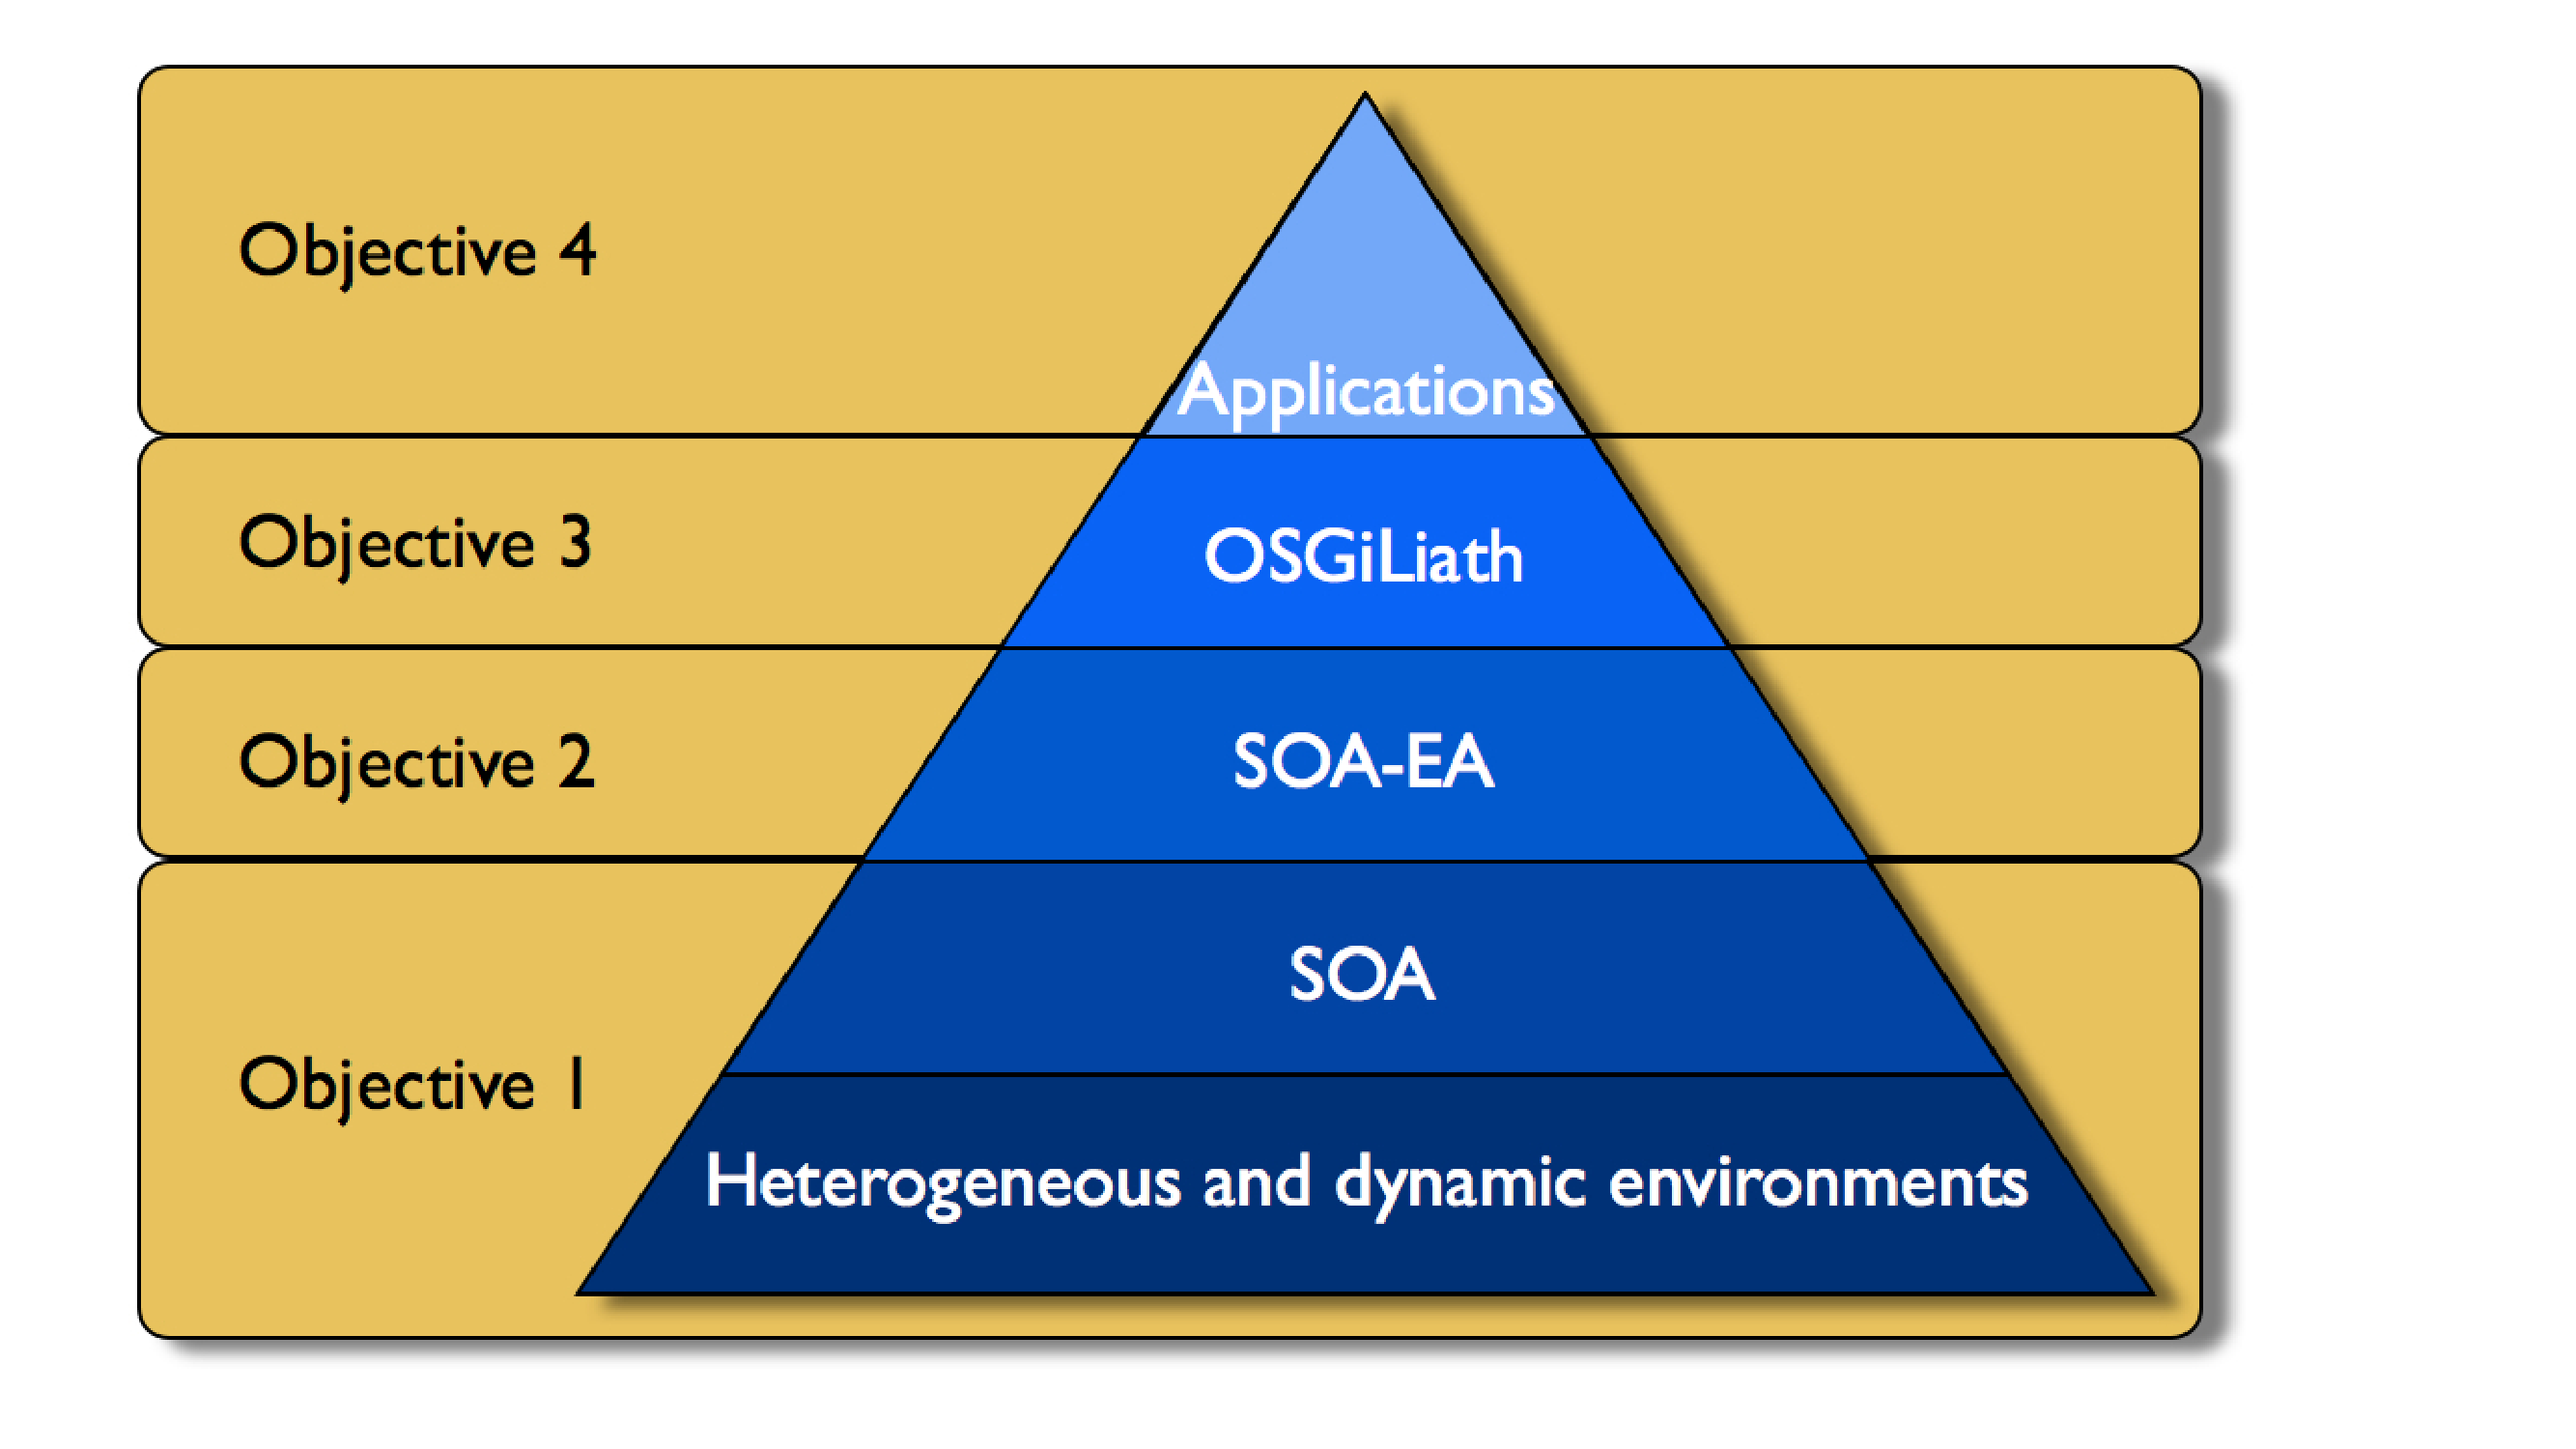
\includegraphics[scale =0.3] {gfx/intro/tesispiramide.pdf}
\caption{Summary of the objectives of this thesis.}
\label{fig:intro:piramid}
\end{SCfigure}

% ESto ya no corresponde a lo de arriba. 